\documentclass{beamer}

%%%%%%%%%%%%%Solarized Theme%%%%%%%%%%%%%%%
\usecolortheme[light,accent=cyan]{solarized}
\beamertemplatenavigationsymbolsempty
%%%%%Packages%%%%%
\usefonttheme{serif}
\usepackage[T1]{fontenc}
\usepackage[utf8]{inputenc}
\usepackage[english]{babel}
\usepackage{fontawesome}
\usepackage{minted}
\usepackage{soul}
\usepackage{ulem}
\usepackage{blkarray}
\usepackage{multirow}
\usepackage[ruled,vlined]{algorithm2e}

\definecolor{DarkGray}{gray}{0.1}
\usemintedstyle{paraiso-dark}


\usepackage{graphicx}
\usepackage{hyperref}
\usepackage{colortbl, xcolor}
\usepackage{booktabs}
\usepackage{amsmath,amsthm, amssymb, latexsym}

\usepackage{tikz}
\usepackage{xcolor}
\usepackage{graphicx,multirow}
\definecolor{plain}{rgb}{93,93,93}
\usetikzlibrary{positioning,arrows}
\definecolor{applegreen}{rgb}{0.55, 0.71, 0.0}
\usetikzlibrary{decorations.pathreplacing, backgrounds, fit,}
\usetikzlibrary{calc,matrix}

\tikzstyle{background}=[solarizedRed, rectangle, draw, inner sep=1mm, thick,
           rounded corners=2mm]

\tikzset{
  treenode/.style = {align=center, inner sep=0pt, text centered,
    font=\sffamily},
  arn_n/.style = {treenode, circle, white, font=\sffamily\bfseries, draw=black, inner sep=-6pt,
    fill=black, text width=1.5em},% arbre rouge noir, noeud noir
  arn_r/.style = {treenode, circle, red, 
    text width=1.5em, very thick, inner sep=4pt},% arbre rouge noir, noeud rouge
  arn_x/.style = {treenode, rectangle, draw=black,
    minimum width=0.5em, minimum height=0.5em}% arbre rouge noir, nil
}

\usepackage{standalone}
\usepackage{siunitx}

\begin{document}

\begin{frame}
    \begin{center}
        \Large{\textcolor{orange}{Reactive-\(n\) strategies of direct reciprocity}} \\
        \vspace{.5cm}

        \vspace{1cm}
        \normalsize{Theory Seminar} \\
        \vspace{.5cm}
        \normalsize{Nikoleta Glynatsi, Christian Hilbe}

    \end{center}
\end{frame}

\begin{frame}
    \centering
    \includestandalone[width=.8\textwidth]{static/iterated_prisoners_dilemma}
\end{frame}

\begin{frame}
    \begin{center}
        \includestandalone[width=.8\textwidth]{static/memory_n} \\
        \vspace{1cm} \pause

        memory-\(n\) strategies
    \end{center}
\end{frame}

\begin{frame}
    \footnotesize{
    \begin{itemize}[<+->]
        \item Press, W.H. and Dyson, F.J., 2012. Iterated Prisoner's Dilemma contains strategies that dominate any evolutionary opponent. Proceedings of the National Academy of Sciences
        \item Glynatsi, N.E. and Knight, V.A., 2020. Using a theory of mind to find best responses to memory-one strategies. Scientific reports
        \item Hilbe, C., Martinez-Vaquero, L.A., Chatterjee, K. and Nowak, M.A., 2017. Memory-n strategies of direct reciprocity. Proceedings of the National Academy of Sciences
        \item Stewart, A.J. and Plotkin, J.B., 2016. Small groups and long memories promote cooperation. Scientific reports
    \end{itemize}}
\end{frame}

\begin{frame}
    \begin{center}
        \includestandalone[width=.45\textwidth]{static/memory_n}\pause
        \includestandalone[width=.45\textwidth]{static/reactive_n}
    \end{center}
\end{frame}

\begin{frame}
    \centering
    Akin, E., 2016. The iterated prisoner's dilemma: good strategies and their dynamics. Ergodic Theory, Advances in Dynamical Systems

    \pause
    \includestandalone[width=.45\textwidth]{static/memory_one}
\end{frame}

\begin{frame}
    \centering
    \includestandalone[width=0.6\textwidth]{static/states}
\end{frame}

\begin{frame}
    \centering
    \includestandalone[width=0.6\textwidth]{static/states_two} \\
    \vspace{1cm}

    \pause
    \(\mathbf{p} = (p_1, p_2, p_3, p_4)\) \& \(\mathbf{q} = (q_1, q_2, q_3, q_4)\) \\
    \vspace{.5cm}
    \pause

    \(\mathbf{v} M = \mathbf{v}\) \\
    \vspace{.5cm}
    \pause

    \(\mathbf{S}_{p} = (b-c, -c, b, 0)\) \& \(\pi(\mathbf{p}, \mathbf{q}) = \mathbf{v} \cdot \mathbf{S}_{p}\)
\end{frame}

\begin{frame}
    \centering
    Akin, E., 2016. The iterated prisoner's dilemma: good strategies and their dynamics. Ergodic Theory, Advances in Dynamical Systems
\end{frame}

\begin{frame}
    \footnotesize{
    \begin{definition}
        A memory-one strategy is \textbf{agreeable} if it always cooperates following a mutual cooperation,
        thus \(p_1=1\).
    \end{definition}}
\end{frame}

\begin{frame}
    \footnotesize{
    \begin{definition}
        A strategy is called \textbf{good} if (i) it is agreeable,
        and (ii) if for any general strategy chosen by the co-player against it the expected
        payoffs satisfy:
        
        \begin{equation}
          s_{\mathbf{q}} \geq (b - c) \Rightarrow s_{\mathbf{q}} = s_{\mathbf{p}} =  (b - c).
        \end{equation}
      
        The strategy is of \textbf{Nash type} if (i) it is agreeable and (ii) if the
        expected payoffs against any general strategy satisfy:
      
        \begin{equation}
          s_{\mathbf{q}} \geq R \Rightarrow s_{\mathbf{q}} =  (b - c).
        \end{equation}
      \end{definition}}
\end{frame}

\begin{frame}
    \begin{theorem}{Akin's Theorem.}
        \begin{align*}
        (1 - p_1) \cdot v_1 + (1 - p_2) \cdot v_2 = p_3 \cdot v_3 + p_4 \cdot v_4
        \end{align*}
    \end{theorem}
\end{frame}


\begin{frame}
    \begin{center}
        \includestandalone[width=\textwidth]{static/two_bit_reactive}
    \end{center}
\end{frame}

\begin{frame}
    \begin{definition}
        A \(n-\)bit reactive strategy is agreeable if it cooperates with a probability one
        given that the co-player has consecutively cooperated in that last \(n\) rounds.
    \end{definition}
\end{frame}

\begin{frame}
    \tiny{
    \begin{lemma}{Extension of Akin's Theorem}
        \begin{align*}
        (v_{1} + v_{9}) (1 - p_1) + (v_{2} + v_{10}) (1 - p_2)  + (v_{5} + v_{13}) (1 - p_3) + (v_{6} + v_{14}) (1 - p_4) \nonumber \\
        = (v_{3} + v_{11})p_1  + (v_{4} + v_{12})p_2 + (v_{7} + v_{15}) p_3 + (v_{8} + v_{16}) p_4.
        \end{align*}
      \end{lemma}}
\end{frame}

\begin{frame}
    \footnotesize{
    \begin{theorem}
        Let the two-bit reactive strategy \(\mathbf{\hat{p}} = (p_{1}, p_{2}, p_{3}, p_{4})\) be an \textbf{agreeable
        strategy}; that is \(p_1 = 1\). Strategy \(\mathbf{\hat{p}}\) is \textbf{Nash} if the
        following inequalities hold:
        \begin{equation*}
            p_4 \leq 1 - \frac{c}{b} \qquad  p_2  \leq p_4 \qquad p_3 \leq 1 \qquad (1 + p_2) \leq \frac{b}{c} - \frac{p_4 (b - c)}{c}
        \end{equation*}
        
        The agreeable strategy \(\mathbf{\hat{p}}\) is good if and only if all inequalities above are strict.
    \end{theorem}}
\end{frame}

\begin{frame}
    \begin{center}
        \includegraphics[width=.65\textwidth]{static/one}
    \end{center}
\end{frame}

\begin{frame}
    \footnotesize{
    \begin{theorem}
        Let the memory-two strategy \(\mathbf{p} = (p_{1}, p_{2}, \dots, p_{16})\) be an \textbf{agreeable
        strategy}; that is \(p_1 = 1\). Strategy \(\mathbf{p}\) is \textbf{Nash} if the
        following inequalities hold:
        \begin{equation*}
            p_2, p_{10}, p_{14}  \leq  p_{6}  \qquad  p_5, p_9, p_{13}  \leq 1 \qquad  \frac{c}{b} p_{11} \leq 1 - p_{6}  \qquad  \frac{c}{b} p_{15} \leq 1 - p_{6} 
        \end{equation*}
        \begin{equation*}
            \frac{c}{b} p_{3} \leq 1 - p_{6}  \qquad  p_6  \leq 1 + \frac{c}{b - c} p_{12} \qquad  p_6  \leq 1 + \frac{c}{b - c} p_{16}
        \end{equation*}
        \begin{equation*}
             \frac{c}{b} p_{7} \leq 1 - p_6  \qquad \frac{c}{b -c} p_{8} < 1 - p_6
        \end{equation*}

        The agreeable strategy \(\mathbf{p}\) is good if and only if all inequalities above are strict.
    \end{theorem}}
\end{frame}

\begin{frame}
    \begin{center}
        \includegraphics[width=.65\textwidth]{static/Ideas_Surprised_Pikachu_HD}
    \end{center}
\end{frame}

\begin{frame}
    \footnotesize{
    \begin{theorem}
        Let the memory-two strategy \(\mathbf{p} = (p_{1}, p_{2}, \dots, p_{16})\) be an \textbf{agreeable
        strategy}; that is \(p_1 = 1\). Strategy \(\mathbf{p}\) is \textbf{Nash} if the
        following inequalities hold:
        \begin{equation*}
            p_2, p_{10}, p_{14}  \leq  p_{6}  \qquad  p_5, p_9, p_{13}  \leq 1 \qquad  \frac{c}{b} p_{11} \leq 1 - p_{6}  \qquad  \frac{c}{b} p_{15} \leq 1 - p_{6} 
        \end{equation*}
        \begin{equation*}
            \frac{c}{b} p_{3} \leq 1 - p_{6}  \qquad  p_6  \leq 1 + \frac{c}{b - c} p_{12} \qquad  p_6  \leq 1 + \frac{c}{b - c} p_{16}
        \end{equation*}
        \begin{equation*}
             \frac{c}{b} p_{7} \leq 1 - p_6  \qquad \frac{c}{b -c} p_{8} < 1 - p_6
        \end{equation*}

        The agreeable strategy \(\mathbf{p}\) is good if and only if all inequalities above are strict.
    \end{theorem}}
\end{frame}

\begin{frame}
    \begin{center}
        \Large Numerical Evaluation of Nash
    \end{center}
\end{frame}

\begin{frame}
    \begin{center}
        \includegraphics[width=.65\textwidth]{static/two}
    \end{center}
\end{frame}

\begin{frame}
    \begin{center}
        \includegraphics[width=\textwidth]{static/three}
    \end{center}
\end{frame}

\begin{frame}
    \begin{center}
        \includegraphics[width=\textwidth]{static/four}
    \end{center}
\end{frame}

\begin{frame}
    \begin{center}
        \includestandalone[width=.5\textwidth]{static/memory_two}
    \end{center}
\end{frame}

\begin{frame}
    \begin{center}
        \includegraphics[width=.65\textwidth]{static/Ideas_Surprised_Pikachu_HD copy}
    \end{center}
\end{frame}

\begin{frame}
    \begin{center}
        \Large 1. Anti Press and Dyson
    \end{center}
\end{frame}

\begin{frame}
    \begin{center}
        \includegraphics[width=.65\textwidth]{static/two}
    \end{center}
\end{frame}

\begin{frame}
    \begin{center}
        \includegraphics[width=\textwidth]{static/five_b}
    \end{center}
\end{frame}

\begin{frame}
    \begin{center}
        \includegraphics[width=\textwidth]{static/six_b}
    \end{center}
\end{frame}

\begin{frame}
    \begin{center}
    Let X play a short memory strategy, and Y play with longer memory of the
    past outcomes. In the perspective of the forgetful strategy X, X's score
    is exactly the same as if Y had played a certain shorter-memory strategy.
    \end{center}
\end{frame}

\begin{frame}
    \begin{center}
    Let X play a memory-one strategy, and Y play a longer memory-\(n\) strategy.
    In the perspective of X, there is a memory-one representation
    of Y's strategy such that X's score is exactly the same.
    \end{center}
\end{frame}

\begin{frame}
    \begin{center}
    Let X play a one-bit reactive strategy, and Y play a longer memory-\(n\) strategy.
    In the perspective of X, there is a memory-one representation
    of Y's strategy such that X's score is exactly the same.
    \end{center}
\end{frame}


\begin{frame}
    \begin{center}
        \Large 2. Pure Nash
    \end{center}
\end{frame}

\begin{frame}
    \footnotesize{
    \begin{theorem}
        Let \(\mathbf{p} = (p_1, p_2, p_3, p_4)\) be an agreeable memory-one strategy. That is, \(p_1 = 1\).
        The strategy \(\mathbf{p}\) is of Nash type iff the following inequalities hold:
        \begin{equation*}
            \frac{c p_3}{b} \leq (1 - p_2)  \qquad \frac{c p_4}{(b - c)} \leq (1 - p_2)
        \end{equation*}
    
        The strategy \(\mathbf{p}\) is good iff, in addition, both inequalities are strict.
    \end{theorem}}
\end{frame}

\begin{frame}
    \begin{center}
        \includegraphics[width=\textwidth]{static/six} \\
        \vspace{.5cm}

        \tiny{Hilbe, C., Martinez-Vaquero, L.A., Chatterjee, K. and Nowak, M.A., 2017. Memory-n strategies of direct reciprocity. Proceedings of the National Academy of Sciences}

    \end{center}
\end{frame}

\begin{frame}
        \centering
        \resizebox{\linewidth}{!}{%
         \begin{tabular}{c c c c c}
        \toprule
         & Strategy & \(\rho\) (self coop. rate) & Min. \(\frac{b}{c}\) ratio & Max. \(\frac{b}{c}\) ratio \\
        \midrule
         \multirow{ 1}{*}{One-bit reactive} & \(p_1 = 0, p_2 = 0\) & 0 & 0 & 0\\
         \midrule
         \multirow{ 2}{*}{Two-bit reactive} & \(p_1 = 0, p_2 = 0, p_3=0, p_4=0\) & 0.0 & None & None\\
         & \(p_1 = 0, p_2 = 1, p_3=0, p_4=0\) & 0.255 & 1.04 & None \\
         & \(p_1 = 0, p_2 = 0, p_3=1, p_4=0\) & 0.255 & 1.04 & None \\
         \midrule
         \multirow{ 3}{*}{Three-bit reactive} &  \(p_1 = 0, p_2 = 0, p_3=0, p_4=0, p_5=0, p_6=0, p_7=0, p_8=0\) & 0.0 & None & None\\
         & \(p_1 = 0, p_2 = 0, p_3=0, p_4=0, p_5=0, p_6=1, p_7=0, p_8=0\) & 0.182 & 1.0590 & 1.0592 \\
         & \(p_1 = 0, p_2 = 0, p_3=1, p_4=0, p_5=0, p_6=0, p_7=1, p_8=0\) & 0.255 & 1.041 & 1.042 \\
         \bottomrule
      \end{tabular}} \\
      \vspace{.5cm}


      \tiny{\textbf{Pure one, two and three bit(s) reactive strategies (\(\epsilon=0.01\)).}}
\end{frame}

\begin{frame}
    \begin{center}
    \faTwitter \ @NikoletaGlyn \\
    \faTwitter \ @chilbe3 \\
    \vspace{1cm}

    \faGithub \ Nikoleta - v3 \\
    http://web.evolbio.mpg.de/social-behaviour/ \\
    \vspace{1cm}

    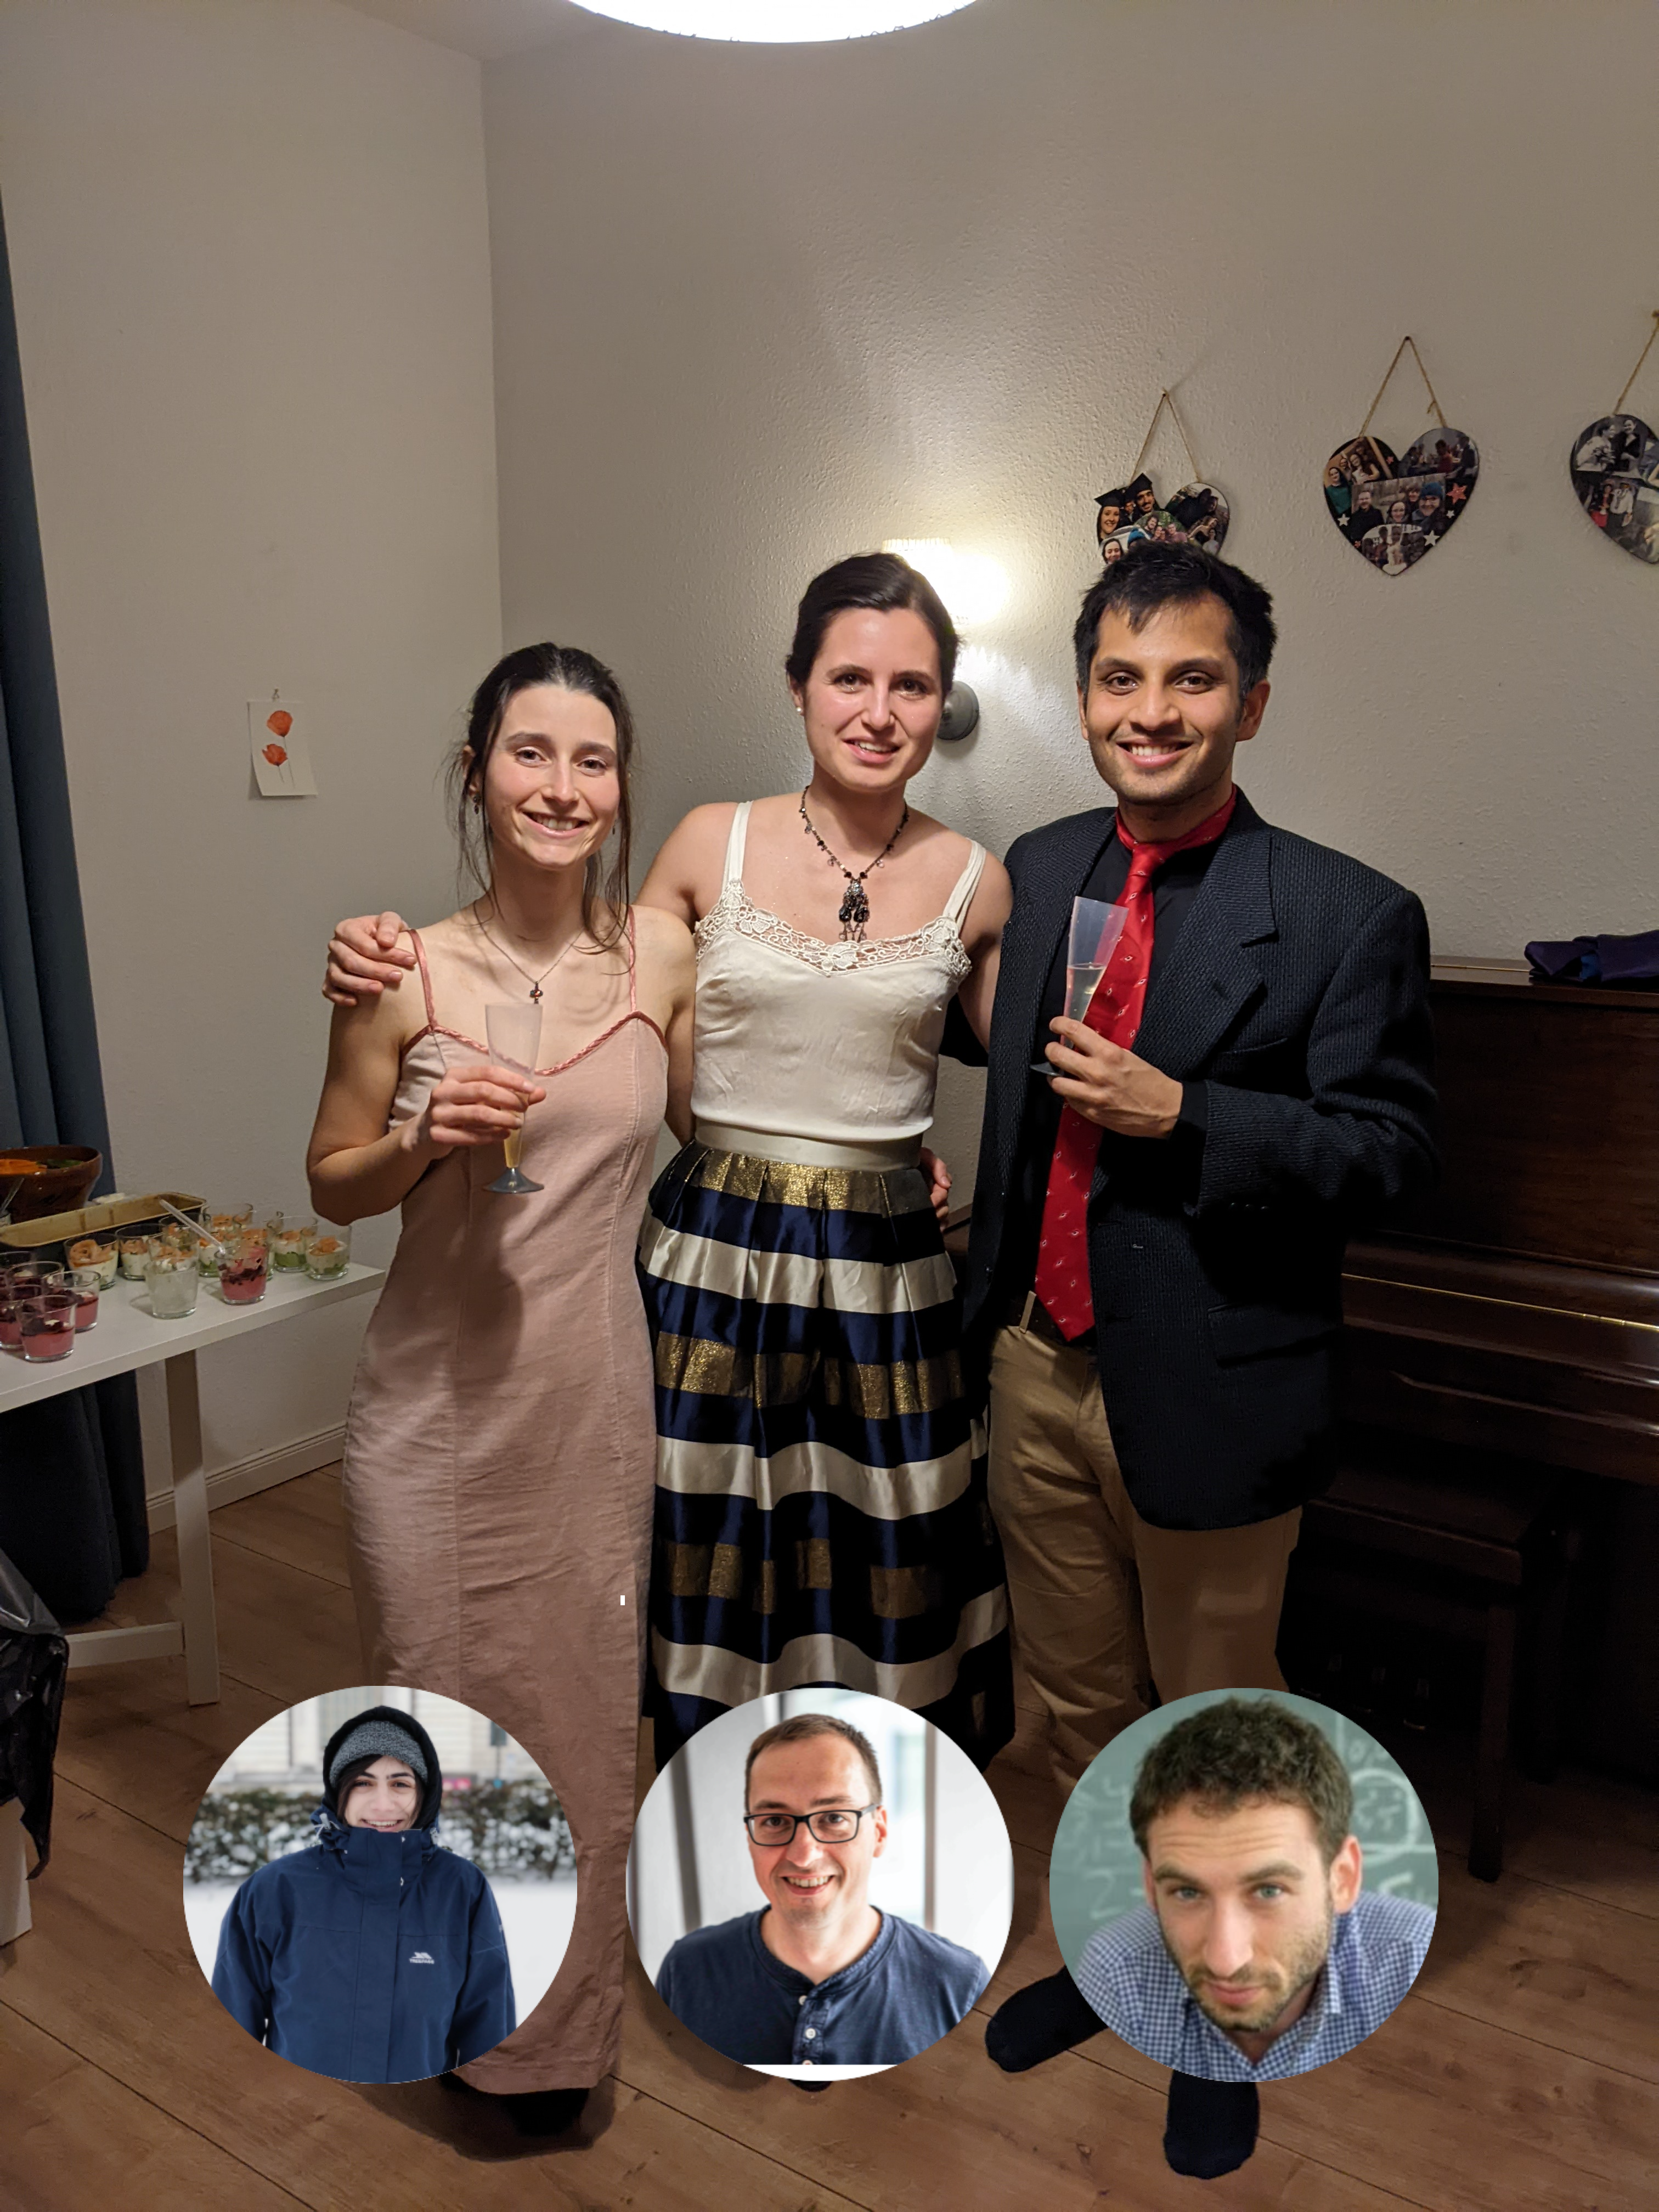
\includegraphics[width=.3\textwidth]{static/Marta's card.png}
    \end{center}
\end{frame}

\begin{frame}
    \begin{center}
        \includestandalone[width=\textwidth]{static/evolution}
    \end{center}
\end{frame}

\begin{frame}
    \begin{center}
        \includegraphics[width=\textwidth]{static/five}
    \end{center}
\end{frame}

\begin{frame}
    \begin{center}
        \includegraphics[width=\textwidth]{static/evolution_results_barplots.pdf}
    \end{center}
\end{frame}



\end{document}